\documentclass[a4paper, 12pt]{article}
\usepackage{temp}
\usepackage{epsfig,graphicx,subfigure,amsthm,amsmath, float, xcolor, changepage, mathtools, textcomp, hyperref, bm, amssymb, tcolorbox, tikz, setspace}
\usepackage{array}
\usepackage[shortlabels]{enumitem}
\usepackage[stable]{footmisc}
\usepackage{xepersian}
\settextfont[Scale=1]{XBZar}
%\setdigitfont{XBZar}
\setlatintextfont[Scale=0.9]{Times New Roman}
\hypersetup{
	colorlinks=true,
	urlcolor=blue!70!black
}

\newcolumntype{?}{!{\vrule width 1pt}}

\doublespacing
\begin{document}
\handout
{هوش مصنوعی}
{نیم‌سال اول ۰۱\lr{-}۰۰}
{دکتر محمدحسین رهبان}
{دانشکده مهندسی کامپیوتر}
{تمرین چهارم - بخش اول}
{محمدجواد هزاره}
{98101074}
\noindent
\\[-6em]
\section*{سوال ۱}
\begin{enumerate}[A)]
	\item
	متغییرهای مسئله را به صورت زیر تعریف می‌کنیم:
	\[
	\begin{dcases}
		\, X := \text{نتیجه پرتاب سکه} 	& \quad X \in \{H, T\} \\
		\, Ball:= \text{نتبجه انتخاب توپ}	& \quad Ball \in \{W, R, B, G\} \\
	\end{dcases}
	\]
	بنابراین با توجه به اطلاعات داده شده برای احتمال $X$ و احتمال $Ball$ به شرط $X$، برای شبکه‌ی بیزی داریم:	
	\begin{figure}[H]
		\centering
		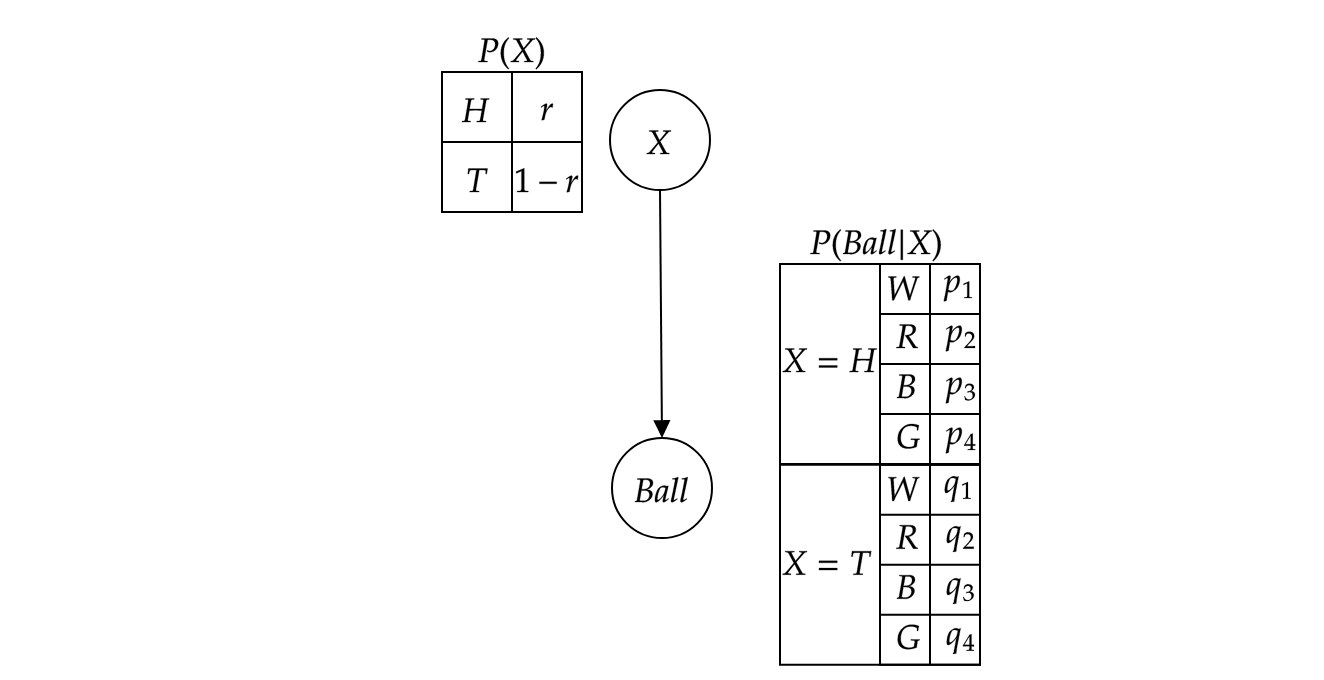
\includegraphics[width=0.8\textwidth]{net.png}
		\caption{شبکه بیزی}
	\end{figure}
	\item
	احتمال این‌که پرتاب اول $H$ و توپ انتخاب شده سفید باشد برابر است با:
	\[
	\prob(X=H, Ball=W) = \prob(X=H)\prob(Ball=W|X=H) = rp_1
	\]
	احتمال این‌که پرتاب دوم $T$ و توپ انتخاب شده سفید باشد برابر است با:
	\[
	\prob(X=T, Ball=W) = \prob(X=T)\prob(Ball=W|X=T) = (1-r)q_1
	\]
	احتمال این‌که پرتاب سوم $T$ و توپ انتخاب شده سفید باشد نیز به طور مشابه برابر با 
	$(1-r)q_1$
	خواهد بود. بنابراین احتمال این‌که هر سه توپ سفید باشند برابر است با
	$rp_1 + 2(1-r)q_1$.
	به طور مشابه احتمال این‌که هر سه توپ قرمز باشند برابر است با
	$rp_2 + 2(1-r)q_2$
	و $\cdots$ .
	بنابراین احتمال این‌که هر سه توپ هم‌رنگ باشند برابر خواهد بود با جمع احتمال این‌که هر سه توپ سفید یا آبی یا قرمز یا سبز باشند، بنابراین:
	\[
	\begin{aligned}
		\prob(\text{هر سه توپ هم‌رنگ}) &= \sum_{i=1}^4 r(p_i) + 2(1-r)q_i \\
		&= r \sum_{i=1}^4 p_i + 2(1-r) \sum_{i=1}^4 q_i\\
		&= \boxed{2 - r} 
	\end{aligned}
	\]
	\item
	با توجه به قانون بیز داریم:
	\[
	\prob(H|R) = \frac{\prob(H)\prob(R|H)}{\prob(R)}
	\]
	برای مخرج کسر با استفاده از قانون احتمال کل داریم:
	\[
	\begin{aligned}
		\prob(Ball=R) = \prob(H)\prob(R|H) + \prob(T)\prob(R|T) = rp_2 + (1-r)q_2
	\end{aligned}
	\]
	بنابراین برای خواسته‌ی مسئله داریم:
	\[
	\boxed{\prob(H|R) = \frac{rp_2}{rp_2 + (1-r)q_2}}
	\]
\end{enumerate}
\end{document}



